\newcommand{\reals}{{\rm I\!\hspace{-0.025em} R}}

\def\A{{\cal A}}
\def\S{{\cal S}}

% +------------------------------------------------------------------------+
\section{Introduction}

The problem of finding all lines that cross four line segments arises
in many fields of computation such as computer graphics (visibility
computations), computer geometry (assembly planning), and computer
vision (object recognition).

The method described in this chapter computes all lines that cross
four line segments taken from a set of $n$ line segments in three
dimensional Euclidean space. The algorithm and its implementation are
robust. The code properly handles all degenerate cases; a line segment
may degenerate to a point; several segments may overlap, be parallel,
coplaner, colinear (lie on the same supporting line), or concurrent
(intersect at a common point.

\begin{figure}
\begin{ccTexOnly}
\centerline{%
  \begin{tabular}{cc}
    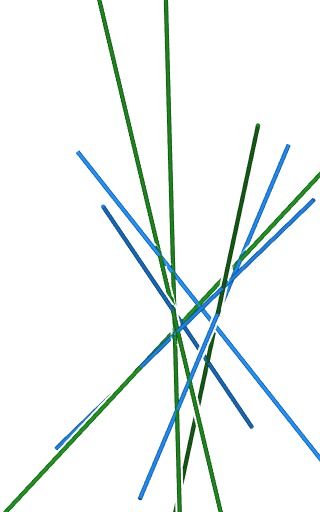
\includegraphics[width=5cm]{Lines_through_segments_3/4_transversals.jpg} &
    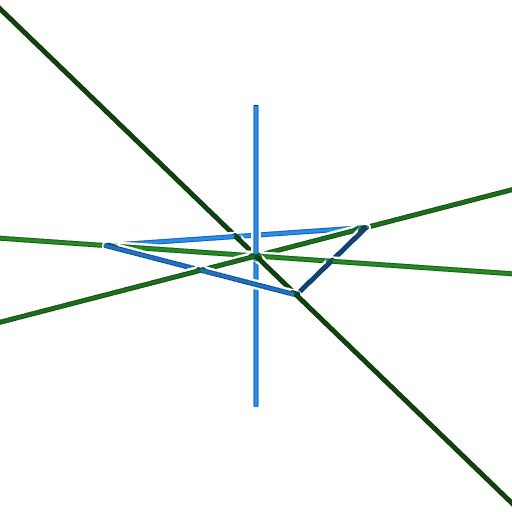
\includegraphics[width=5cm]{Lines_through_segments_3/3_transversals.jpg}\\
    (a) & (b)
  \end{tabular}
}
\end{ccTexOnly}
\label{fig:intro}
\begin{ccHtmlOnly}
<P>
<center>
<table>
<tr align="center">
<td><img src="4_transversals.jpg" border=0 alt="4_transversals"></td>
<td><img src="3_transversals.jpg" border=0 alt="3_transversals"></td>
</tr>
<tr align="center"><td>(a)</td><td>(b)</td></tr>
</table>
</center>
\end{ccHtmlOnly}
\begin{center}
\caption{(a) Four lines (green) that cut across four line segments (blue).
  (b) Three lines (green) that cut across four line segments (blue).}
\end{center}
\label{fig:transversal-3-4}
\end{figure}

The number of lines that cross four arbitrary lines in $\mathbb{R}^3$ is
0, 1, 2, or infinite. When segments are replaced by lines, the number of
transversal lines can be 0, 1, 2, 3, 4, or infinite.
Figure~\ref{fig:transversal-3-4}a shows a case where three lines cross
four segments, and Figure~\ref{fig:transversal-3-4}b shows a case where
four lines cross four segments.

\begin{figure}
\begin{ccTexOnly}
\centerline{%
  \begin{tabular}{ccccc}
    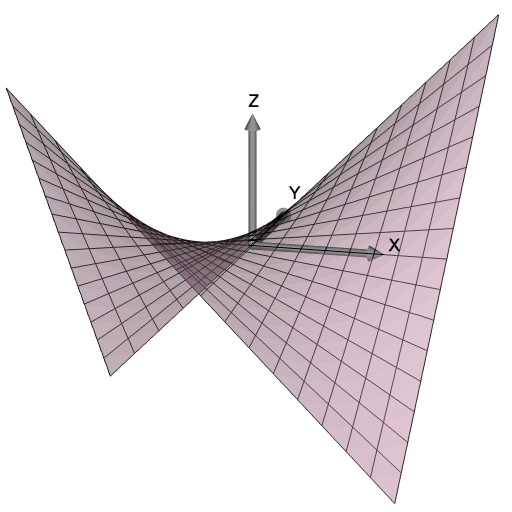
\includegraphics[width=4cm]{Lines_through_segments_3/hyperbolic_paraboloid.jpg} &
    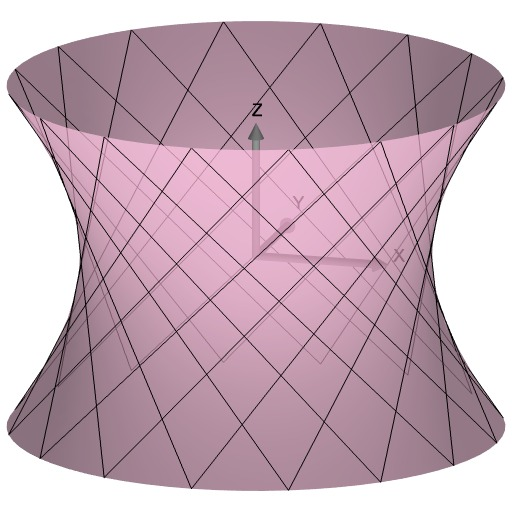
\includegraphics[width=4cm]{Lines_through_segments_3/hyperboloid_of_one_sheet.jpg} &
    
\includegraphics[width=4cm]{Lines_through_segments_3/3_lines_concurrent.jpg} &
    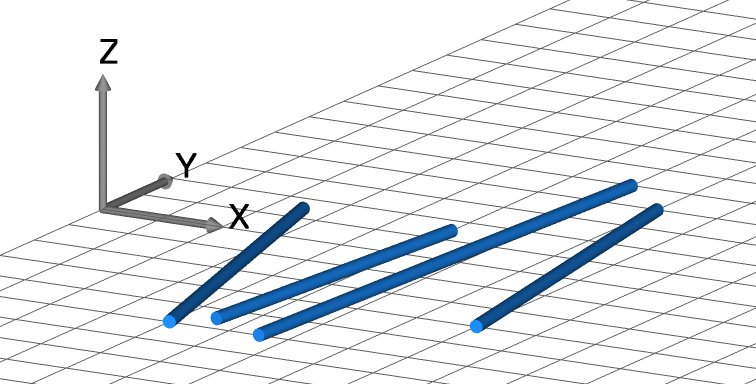
\includegraphics[width=4cm]{Lines_through_segments_3/4_coplanar.jpg} &
    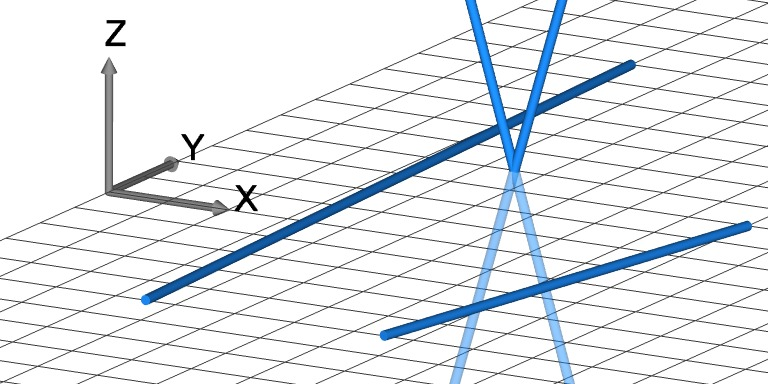
\includegraphics[width=4cm]{Lines_through_segments_3/4_lines_2_meet_on_the_plane.jpg}\\
    (a) & (b) & (c) & (d) & (e)
  \end{tabular}
}
\end{ccTexOnly}
\label{fig:intro}
\begin{ccHtmlOnly}
<P>
<center>
<table>
<tr align="center">
<td><img width="200" src="hyperbolic_paraboloid.jpg" border=0 alt="hyperbolic_paraboloid"></td>
<td><img width="200" src="hyperboloid_of_one_sheet.jpg" border=0 alt="hyperboloid_of_one_sheet"></td>
<td><img width="200" src="3_lines_concurrent.jpg" border=0 alt="3_lines_concurrent"></td>
<td><img width="200" src="4_coplanar.jpg" border=0 alt="4_coplanar"></td>
<td><img width="200" src="4_lines_2_meet_on_the_plane.jpg" border=0 alt="4_lines_2_meet_on_the_plane"></td>
</tr>
<tr align="center"><td>(a)</td><td>(b)</td><td>(c)</td><td>(d)</td><td>(e)</td></tr>
</table>
</center>
\end{ccHtmlOnly}
\begin{center}
\caption{Five cases where the number of lines that cross arbitrary
  four lines (or line segments) in $\mathbb{R}^3$ is infinite.}
\end{center}
\label{fig:transversals-infinite}
\end{figure}

The number of lines that cross arbitrary four lines (or line segments)
in $\mathbb{R}^3$ is infinite when the line segments lie in one of the
following configurations:
\begin{enumerate}
\item%hyperbolic_paraboloid
  The four line segments are all contained in the lines of one ruling of
  hyperbolic paraboloid; see Figure~\ref{fig:transversals-infinite}a.
\item%hyperboloid_of_one_sheet
  The four line segments are all contained in the lines of one ruling of
  hyperboloid of one sheet; see Figure~\ref{fig:transversals-infinite}b.
\item%concurrent
  Three of the line segments are concurrent; see
  Figure~\ref{fig:transversals-infinite}c.
\item%coplanar
  The four line segments are coplanar; see
  Figure~\ref{fig:transversals-infinite}d. 
\item%4_lines_2_meet_on_the_plane
  Two of the line segments lie on a plane, the second two line segments
  meet the plane at the same point; see
  Figure~\ref{fig:transversals-infinite}e.
\end{enumerate}

\section{Algorithm Details.}
In this section, we explain the fundamentals of the problem.\newline
The input to the program is a set $S=\{s_1,\ldots,s_n\}$ of $n$ line segments.\newline
Given 3 disjoint skew line segments in 3D Euclidean space $S_1$, $S_2$, and $S_i$, a line L tangent to these 3 line segments has 1 degree of freedom.\newline
We cast the problem into two dimensional parameter plane, in which the supporting line of $S_1$ is parametrized to the x-axis, the supporting line of $S_2$ is parametrized to the y-axis, and $S_i$ is represented by a bounded hyperbola on the parameter plane.
Since $S_1$ and $S_2$ are line segments, only the square ([0,0] [1,1]) is relevant. Each point on the square represents a tangent line to $S_1$ and $S_2$. Each point on the hyperbola inside the square ([0,0], [1,1]) represents a tangent line to $S_1$, $S_2$ and $S_i$.

Each two line segments $S_i$, $S_j$, $j>i$ are parametrized to an arrangement on plane. For each line segment $S_k$ $k>j$  a bounded hyperbola is added to the arrangement. The intersection points between these hyperbolas inside the bounded square represent tangent lines to 4 segments.

\subsection{Degenerate cases.}
When $S_i$ and $S_j$ intersect 2 parameter spaces are used.
\begin{enumerate}
\item A sphere - The sphere center is the intersection point of $S_i$ and $S_j$. Each point on the sphere represents a tangent line to the intersection point of $S_i$ and $S_j$. A segment $S_k$, is parametrized as 2 bounded arcs on the sphere. Each point on the arc represents a tangent line to $S_i$, $S_j$, and $S_k$.  Since the arcs are symmetric, only the upper half of the sphere is used by the algorithm.\newline
For each line segment $S_k$ one or two arcs are added to the upper half of the sphere arrangement. The intersection points between these arcs represent a tangent line to 2 segments and the intersection point of $S_i$ and $S_j$.
%%TODO picture of a sphere (can take the example of the rectangle)
\item
A plane - Since $S_i$ and $S_j$ intersect, they are lying on the same plane P. A tangent line to $S_i$, $S_j$ must lie on P. Hence, for each line segment $S_k$ only the intersection object with P is relevant.
If $S_k$ intersect with P at a point, a bounded hyperbola or a line segment is added to the plane arrangement. Otherwise $S_k$ is contained at P, and up to four faces are added to the arrangement, each point on the face represents a tangent line to $S_i$, $S_j$ and $S_k$.
When 2 faces created by two different line segments $S_k$, $S_l$ overlap, the overlapping face is returned to the output container as bounded polygon. At this case infinite lines passes through to $S_i$, $S_j$, $S_k$ and $S_l$. See the pink faces at figure \ref{fig:img0}.
At each face a counter of the number of overlap faces is maintained. The underlie curve of each edge between two faces with counters $>= 1$, also represents infinite lines that passes through 4 or more segments. See blue curves at figure \ref{fig:img0}.
\end{enumerate}

\begin{figure}
\begin{ccTexOnly}
\centerline{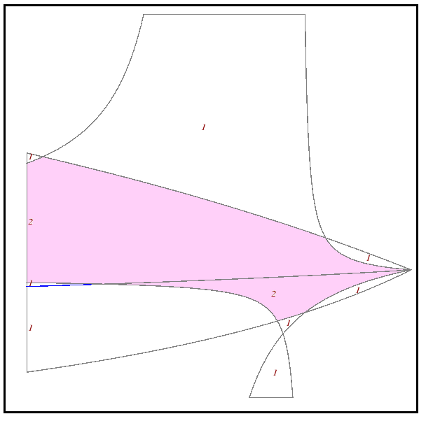
\includegraphics[width=10cm]{Lines_through_segments_3/img0}}
\end{ccTexOnly}
\label{fig:img0}
\begin{ccHtmlOnly}
<P>
<center>
  <img src="img0.png"  border=0 alt="arrangement">
</center>
\end{ccHtmlOnly}
\caption{An arrangement created by five segments, four co-planer and the last, crosses the plane.}
\end{figure}

When $S_i$ and $S_j$ are co-planer, I.e $S_i$, and $S_j$ are parallel, or the supporting lines of $S_i$, and $S_j$ intersect. An arrangement on plane is created, just as the second arrangement when $S_i$ and $S_j$ are intersecting. 

Theoretical bounds for the algorithm are $O((n^3 + K)log n)$ running time, and $O(n^2 + K)$ working storage. Where n is the input size and K is the output size(K is bounded by $n^4$).

\section{Software Design}
The class \ccc{CGAL::Lines_through_segments_3<Lines_through_segments_traits_3>} is parametrized by a traits class which models the concept \ccc{CGAL::LinesThroughSegmentsTraits_3< Rational_kernel, Alg_kernel>}.\newline
The class is a functor, which gets as input an input iterator of line segments, an insert iterator for the output container of output objects, and algebraic and rational kernels for the kernel operations.
The precise description of the requirements is given by the concept \ccc{LinesThroughSegmentsTraits_3}. The class \ccc{CGAL::Lines_through_segments_traits_3} is a model of this concept.

{\bf Output container}\newline
The output objects are of the following types:
\begin{itemize}
\item
\ccc{CGAL::Lines_through_segments_output_line_3} - A tangent line to 4 segments.
\item
\ccc{CGAL::Lines_through_segments_output_arr_curve_2} - A curve on one the plane arrangement. Each point on the curve represents a tangent line to 4 line segments.
The class contains the curve, and pointers to the two rational lines that created the arrangement from which the curve was generated.
\item
\ccc{CGAL::Lines_through_segments_output_arr_arc_2} - An arc on the sphere arrangement. Each point on the arc represents a tangent line to 4 line segments.
The class contains the arc, and pointers to the two rational lines that created the arrangement from which the curve was generated.
\item
\ccc{CGAL::Lines_through_segments_output_arr_polygon_2} - A face on the plane arrangement,  each point on the curve represents a tangent line to 4 line segments.
The class contains the face as \ccc{General_polygon_2}, and pointers to the two rational line segments that created the arrangement from which the polygon was generated.
\item
\ccc{CGAL::Lines_through_segments_output_point_3} - An intersection point of 4 or more concurrent line segments.
The class contains the point as \ccc{Rational_kernel::Point_3}.
\item
\ccc{CGAL::Lines_through_segments_output_overlap_segment_3} - A common line segment to four or more overlapping line segments.
The class contains the line segment as \ccc{Rational_kernel::Segment_3}.
\end{itemize}


\section{Four Line Segment Example}
The following example find all the tangent lines to 4 segments.

\ccIncludeExampleCode{Lines_through_segments_3/lines_through_4_segments.cpp}

This program generates 3 lines, each passes through a vertex of the triangle and the perpendicular segment. The exact output follows:

\begin{verbatim}
Output 1:

Line 1:
   CGAL_LTS_OUTPUT_LINE_3 =  
   6897.60 -5150.99 -1625.33 -6878.34 5155.31 1625.33  
   S1 =  = -2 12 0 11 1 0
   S2 =  = -2 -5 0 11 3 0

Output 2:

Line 1:
   CGAL_LTS_OUTPUT_LINE_3 =  
   4. -1207.00 -719.000 4. 1213.00 733.000
   S1 =  = 2 1 5 4 3 7
   S2 =  = 4 3 7 6 10 12

Line 2:
   CGAL_LTS_OUTPUT_LINE_3 =  
   -16. -32. -22. 20. 34. 32.
   S1 =  = 2 1 5 4 3 7
   S2 =  = 4 3 7 6 10 12

Line 3:
   CGAL_LTS_OUTPUT_LINE_3 =  
   -15. -46. -30. 21. 50. 42.
   S1 =  = 2 1 5 4 3 7
   S2 =  = 4 3 7 6 10 12
\end{verbatim}

% EOF
